
\section{SEAM4US project}
\label{subsec:seam4us}

To investigate on energy efficient subsystems, the EU funded in the Seventh Framework Programme the project "Sustainable Energy mAnageMent for Underground Stations" (SEAM4US).
The aim of SEAM4US "is to develop advanced technologies for optimal and scalable control of metro stations [...]. The project's main outcomes will be the creation of systems for optimized integrated energy management..."~\cite{SEAM4US_Website}.
The integrated energy management is realized by using passenger density models and thermal models, integrating sensors and control algorithms. All models and algorithm compose a model predictive control architecture~\cite{ansuini_models_2013}. The control architecture proactively controls the metro station surroundings (ventilation, escalator, and lightning) under different occupancy and thermal conditions.

The SEAM4US consortium consists of nine partners from six different EU countries, namely Cofely, UniVPM, UPC, Fraunhofer FIT, VTT, Almende, Uni Kassel, CNET and TMB. Each partner supports the consortium within its expertise:

\begin{description}
  \item[Cofely] Cofely Italia Spa (Italy):\\A major player in energy-efficient system management sector
  \item[UniVPM] Universita Politecnica Delle Marche (Italy):\\Building and environmental physics and construction.
  \item[UPC] Universitat Politecnica De Catalunya (Spain):\\Building and environmental physics and construction.
  \item[Fraunhofer~FIT] Fraunhofer-Gesellschaft zur Foerderung der Angewandten Forschung E.V (Germany):\\R+D experts in middleware.
  \item[VTT] Teknologian Tutkimuskeskus VTT (Finland):\\R+D experts in middleware.
  \item[Uni Kassel] University of Kassel (Germany):\\User and agent-based scheduling modeling.
  \item[Almende] Almende B.V. (Netherlands):\\User and agent-based scheduling modeling.
  \item[CNet] CNet Svenska AB (Sweden):\\System integrator.
  \item[TMB] Metropolita De Barcelona Sa (Spain):\\Metro network operator.
\end{description}


%A overview over the SEAM4US consortium is given in Table~\ref{tab:SEAM4USconsortium}.

%\begin{table}[htbp]
%  \centering
%  
%    \begin{tabularx}{\columnwidth}{|X|c|}
%	\hline
%    \textbf{Name} & \textbf{Country} \\
%	\hline
%    Cofely Italia Spa & Italy \\
%	\hline
%    Universita Politecnica Delle Marche & Italy \\
%	\hline
%    Universitat Politecnica De Catalunya & Spain \\
%	\hline
%    Fraunhofer-Gesellschaft Zur Foerderung Der Angewandten Forschung E.V & Germany \\
%	\hline
%    Teknologian Tutkimuskeskus VTT & Finland \\
%	\hline
%    Universitaet Kassel & Germany \\
%	\hline
%    Almende B.V. & Netherlands \\
%    	\hline
%    CNet Svenska AB & Sweden \\
%    	\hline
%    	Metropolita De Barcelona Sa & Spain \\
%	\hline
%    \end{tabularx}%
%    
%  \caption{SEAM4US consortium}%
%  \label{tab:SEAM4USconsortium}%
%\end{table}%


\section{Metro Station "Passeig de Gr\`{a}cia"}
\label{sec:station}

%TODO http://www.tmb.cat/en/detall-linia-metro/-/linia/L3/327

The developed technologies were implementation in one of the underground stations of the TMB metro network in Barcelona. This section describes the "station" in detail, while the word "station" in the area of metro networks needs to be defined first.

A metro network is consist of one or more metro lines. Each line has a defined railway with a given number of stops to allow people to get on or off the trains by means of a platform. Each of these stops is called "line station". In contrast a "metro station" is the concept that represents the point in space through which a passenger gets underground and into a line station. Metro station and line station can be the same physical entity, but it is possible that a "metro stations" consists of one ore ore "line stations".

The metro station Passeig de Gr\`{a}cia~(PdG) is a station within the metro network of TMB and lies in a very iconic and touristic part of Barcelona. Some popular buildings designed by Antoni Gaud\'{i} are in the proximity (Casa Batll\`{o}, Casa Mil\`{a}), as well as the city's most renown and exclusive boutiques.
The metro station is one of the oldest of the Barcelona metro network. First opened in December 1924, as a (line) station for Line~3, nowadays PdG holds three different line stations: L2, L3, and L4. The stations were built in three different periods and using different construction technologies. All line stations has been refurbished a few times since 1924 and new equipment has been added recently. Figure~\ref{fig:PdG_entranceExit} depicts a entrance of metro station Passeig de Gr\`{a}cia.

\begin{figure}[htbp]
  \centering
  \includegraphics[width=\linewidth]{Figures/PdG-L3_entranceExit.jpg} 
  \caption{Passeig de Gr\`{a}cia Entrance/Exit Gran Via. \cite{TMB_2014}}
  \label{fig:PdG_entranceExit}
\end{figure}

Depending on the weekday PdG is open 19~hours, 21~hours or 24~hours. Between Monday and Thursday PdG service starts at 5:00 and ends at 24:00 (19~hours). Friday service starts at 5:00 and ends at 2:00 (21~hours). On Saturday service starts at 5:00 too but remain the entire night and day until Sunday midnight.

The developed technologies were implementation line station in Passeig de Gr\`{a}cia - Line~3~(PdG-L3). In the following all information are respective to PdG-L3.

Passeig~de~Gr\`{a}cia - Line~3~(PdG-L3) turns out to be representative for many station within TMBs metro network~\cite{TMB}. Moreover PdG-L3 is a crowded station which have low-rate usage hours as well. This provides a wide range of data which allows to test with very busy peak hours as well as with off-peaks.

The line station PdG-L3 consists of private (staff only) and public spaces. Private spaces such as technical rooms or staff dependencies are not part of the investigation of the SEAM4US project. Public spaces, such as halls, transit areas, accesses to the platforms, and platforms are however in the focus.

Essential part of (every) line station are the platforms, which allow passengers to leave and enter trains. PdG-L3 laid out on a PRRP (Platform-Rail-Rail-Platform) schema. The PdG-L3 platforms are visible on Figure~\ref{fig:PdG-L3_platforms}. To leave the platform several escalators are available. Figure~\ref{fig:PdG-L3_escalator} depicts exemplary an escalator.

\begin{figure}[htbp]
  \centering
  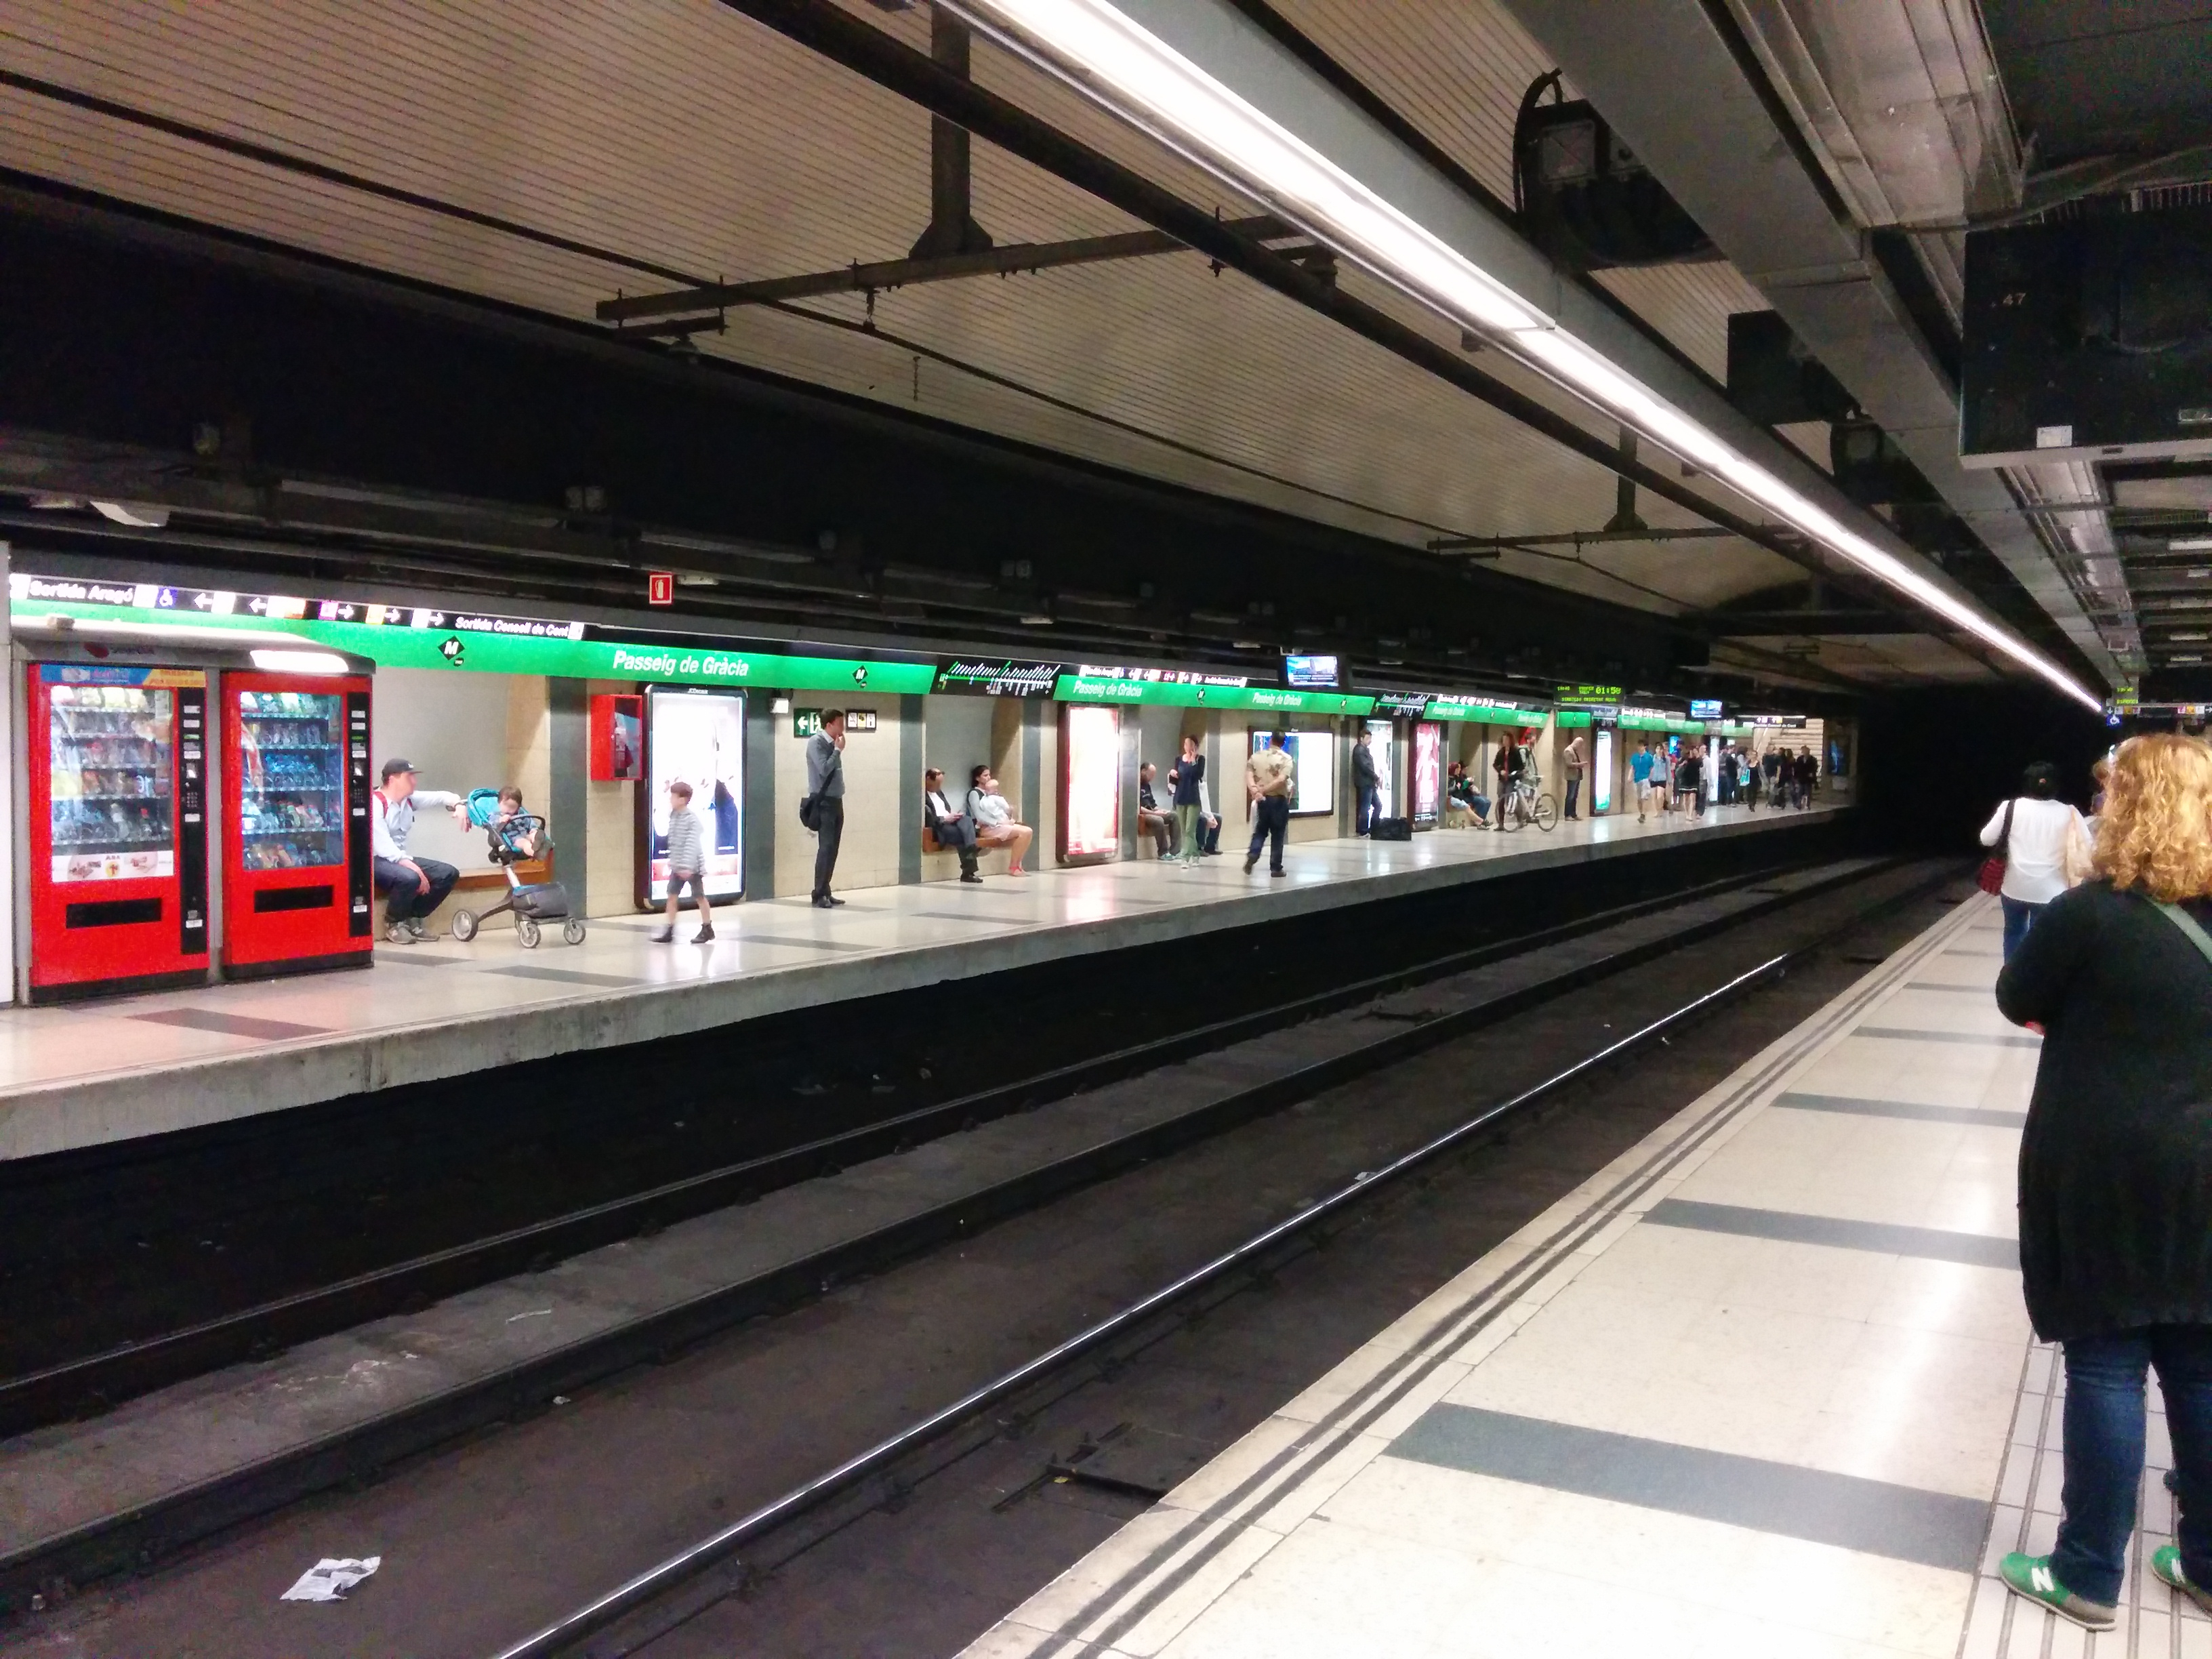
\includegraphics[width=\linewidth]{Figures/PdG-L3_platform.jpg} 
  \caption{PdG-L3 Plattforms. \cite{TMB_2014}}
  \label{fig:PdG-L3_platforms}
\end{figure}

\begin{figure}[htbp]
  \centering
  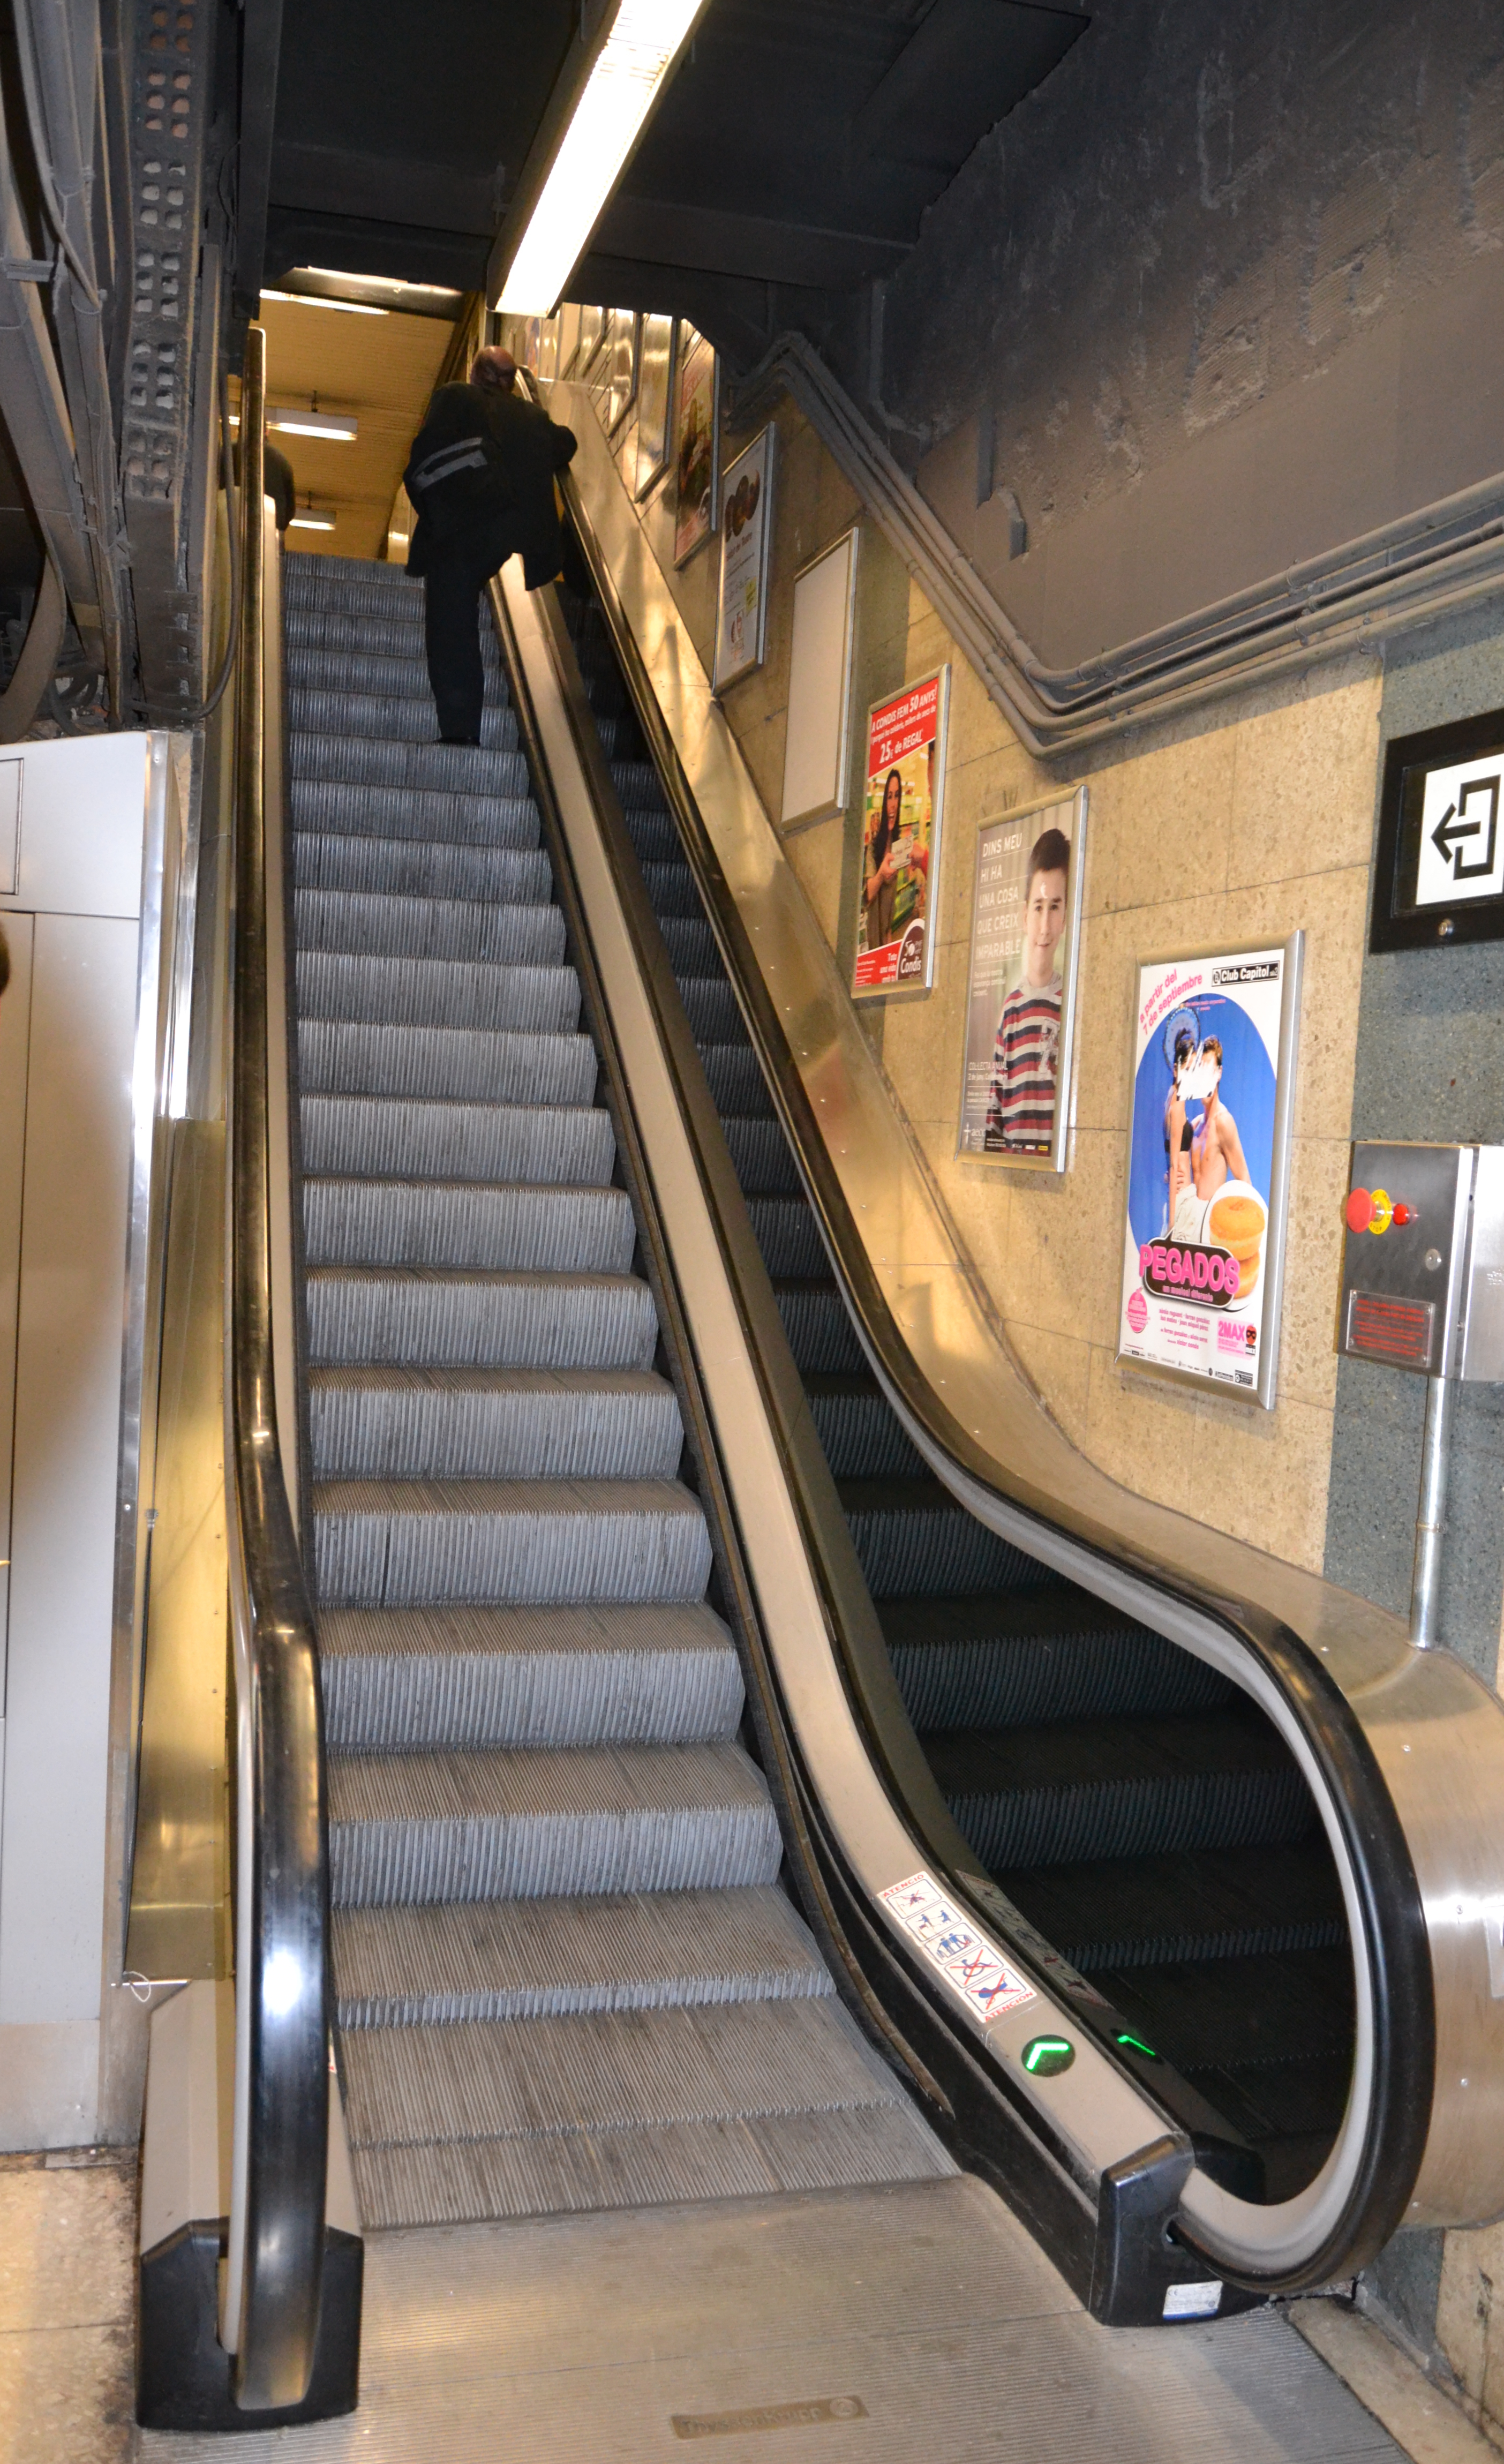
\includegraphics[width=\linewidth]{Figures/PdG-L3_escalator.jpg} 
  \caption{Escalator in PdG-L3 for leaving the platform. \cite{TMB_2014}}
  \label{fig:PdG-L3_escalator}
\end{figure}

A schematic representation of PdG-L3 is drawn in Figure~\ref{fig:PdG-L3_schematic}, where the platforms are highlighted in red. At the beginning and end of the platforms the accesses to the platforms are visible.

\begin{figure}[htbp]
  \centering
  \includegraphics[width=\linewidth]{Figures/PdG-L3_schematic2.jpg} 
  \caption{Schematic representation of PdG-L3. The platforms are highlighted in red. \cite{TMB}}
  \label{fig:PdG-L3_schematic}
\end{figure}

Throughout the station a Closed Circuit Television~(CCTV) surveillance system is installed. 20~CCTV~cameras provides images for security reasons. Figure~\ref{fig:PdG-L3_CCTVcameras} show exemplary CCTV cameras on the platform~(Figure~\ref{fig:PdG-L3_CCTVcamera_transitArea}) as well as in the transit area~(Figure~\ref{fig:PdG-L3_CCTVcamera_transitArea}).

\begin{figure*}[htbp]

  \centering

  \subfigure[CCTV camera installed in a PdG transit area. \cite{TMB_2014}] {
    \includegraphics[width=0.46\textwidth]{Figures/PdG-L3_CCTVcamera_transitArea.jpg}
    \label{fig:PdG-L3_CCTVcamera_transitArea}
  }
  \hfill
  \subfigure[CCTV camera installed in PdG-L3 platform. \cite{TMB_2014}] {
    \includegraphics[width=0.46\textwidth]{Figures/PdG-L3_CCTVcamera_platform.jpg}
    \label{fig:PdG-L3_CCTVcamera_platform}
  }

  \caption{Passenger density distribution of one CCTV camera in PdG-L3.}
  \label{fig:PdG-L3_CCTVcameras}

\end{figure*}


\subsection{Passenger density data extraction}
\label{sec:PassengerDensityDataExtraction}

One part of the predictive controller is the passenger density model. The passenger density model is based on real density seen by the CCTV cameras. Therefore the CCTV~system is reused and enhanced with image processing in order to extract the passenger density within the station. The image processing is described briefly in section.

Whenever camera pictures are processed privacy issues are tackled. In order to ensure the passengers privacy several design constrained where defined:

\begin{enumerate}
  \item All CCTV images are processed within the station.
      \item All CCTV images are processed "on the fly". For the purpose of level of passenger density extraction no CCTV image is saved.
  \item The image processing is performed on a separate computer, which is not connected to other TMB Systems and is only accessible via a dedicated VPN connection.
  \item The image processing works without human interaction.
  \item The image data are filtered to avoid recognisability of individuals.
  \item The image processing results are transmitting only in terms of integer numbers to the database.
\end{enumerate}

With respect to these design constrains the passenger density extraction was implemented. The work flow is described in the following.

First, the video streams coming from all cameras are combined into one single video stream by a video recorder. This video recorder creates a carousel video composed of sections for the individual camera appearing in a predefined order. The duration of the camera sections is set to 3~seconds. With 20~cameras and 3~seconds hold on each, one turn of the carousel is completed in about one minute.

The video recorder is connected to the local computer and transfer the images subsequently. On the local computer the density estimator processes the transferred images and extracts the passenger density.

The density estimator algorithms use a combination of edge detection and background subtraction. In the  following the algorithm is described briefly.
First the algorithm separates background and foreground. Followed by creating the foreground mask.
Through filtering the edges of the foreground only are extracted. The foreground edges are combined with the foreground mask. Finally the result is refined by dilating (and then eroding) the segmented the blobs. %TODO reference ?Almende?
%In parallel to the process described above, we detect the edge of the whole image by applying the Canny edge detection on the three RGB channels of the original image; the results acquired the different channels are then combined via a simple logic OR. Eventually, the intersection of this image with the dilated foreground mask  (obtained using a logic AND) allows us to extract the edges of the foreground only (see Figure 13). 
%"The last step of the crowd density detection algorithm consists in combining this last image with the foreground mask via a logic OR and to refine the result by dilating (and then eroding) the segmented the blobs."  
%All parts have been developed using the C++ OpenCV libraries.
For different reasons, e.g. occluded or damaged camera, it is possible that the crowd density estimator fails. In this case the image processing return the error value "-1".
Finally the extracted passenger density level as well as date, time and the camera-ID of the image are transmitted to the database. The general approach is depicted in Figure~\ref{fig:CCTVimageProcessing}.
%The results transmitted to a three~dimensional database, which holds information about the number of passenger, the location and the time.

\begin{figure}[htbp]
  \centering
  \includegraphics[width=\linewidth]{Figures/imageProcessing.pdf} 
  \caption{Gathering number of people out of the camera images.}
  \label{fig:CCTVimageProcessing}
\end{figure}

The CCTV and image processing runs 24~hours, 7~days a week. Each day 28800~datasets are transmitted to the database. Overall the database contains 90~days of data. The available data are discussed in the next section.

